\chapter{Introduction}\label{ch:introduction}
\section{Optimization}

Improvement means finding better solutions to problems.  These problems may be to win a game \cite{re:mri}\cite{re:lightbot}.  Any system for which the quality of a  function.\footnote{Some objective functions make the goal minimization rather than maximization, but the process is effectively the same.}  Some situations require  method is the Genetic Algorithm, the subject of this work.  

The simplest optimization method is to examine every solution in the search space, to compute, time is often given in iterations rather than seconds.

\subsection{Mastermind}
Consider a simple code-breaking game to be referred to henceforth as Mastermind \cite{re:mastermind}.  The objective of the player is to guess a multi-digit sort of difficult problem for which approximate optimization is often used \cite{re:knuth}\cite{re:stuckman}.

The objective function is defined in equation 1.  The motivation behind it will be explained in section~\ref{sec:evolutionaryheuristics}.
	\begin{equation}
		\label{eq:mastermindfitness}
		f(code) = correct + log(partially correct)
	\end{equation}

\subsection{Random Search}
Another obvious optimization method would be to repeatedly guess while keeping probability of having found the optimum in $k$ trials given a search space of size $n$ given by the following equation and shown for various values of $n$ in Figure~\ref{fig:randomsearchprobability}.  
 
	\begin{equation}
		p(k|n) = 1 - \left(1 - \frac{1}{n}\right)^k
	\end{equation}
	
Given the probability of guessing the solution in $n$ trials is approximately 63\%the objective function for random search is shown in Figure~\ref{fig:randomsearchquality}, normalized to 1 for the maximum possible value.  This shows that, while 

	
	\begin{figure}
		\begin{center}
			\scalebox{0.7}{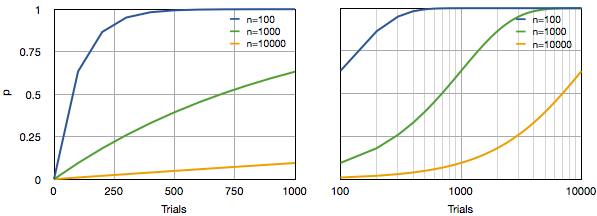
\includegraphics{RandomSearchProbability}} 
		\end{center}
	\caption{Probability of having guessed optimal solution in $k$ trials given search size $n$, for $n$=100, 1000, and 10000.}
	\label{fig:randomsearchprobability}
	\end{figure}

	\begin{figure}
		\begin{center}
			\scalebox{0.80}{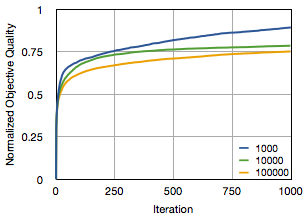
\includegraphics{RandomSearchQuality}} 
		\end{center}
	\caption{Normalized objective function quality for random search of Mastermind for $k$ iterations given search size $n$=100, 1000, 10000.  Averaged over 1000 trials.}
	\label{fig:randomsearchquality}
	\end{figure}

Most evolutionary algorithms include notions of a population, a fitness function, a selection method, and a breeding method \cite{re:evolutionaryalgorithms}.  The population contains potential solutions to an optimization problem, the quality of which is judged by the fitness function.  A generic evolutionary algorithm is shown in Table~\ref{tab:genericevultionaryalgorithm}.

	\begin{table}
		\caption{Generic Evolutionary Algorithm} \hline
		\label{tab:genericevultionaryalgorithm}
		% \begin{tabular}{0.75\textwidth}{l}
		\begin{tabular}{l} \\
		population \(\gets\) random initial values \\ \\
		WHILE fitness of best population member \(\leq\) required fitness \\ \\
			\tab new\_population \(\gets\) empty list\\ \\
			\tab REPEAT \\ \\
				\tab \tab Select parents from the population proportionally to fitness \\ \\
				\tab \tab Breed parents to create children. \\ \\
				\tab \tab Add children to new\_population. \\ \\
			\tab UNTIL size(new\_population) == size(population) \\ \\
			\tab population \(\gets\) new\_population \\
		\end{tabular}
		\hline
	\end{table}
	

A more specific version of evolution is genetic evolution, which treats the gene as the main element of evolution rather than the organism \cite{re:selfishgene}.  of genes, and the breeding methods should be akin to genetic crossover and mutation.  

\subsection{Heuristics} \label{sec:evolutionaryheuristics}
A major way in which algorithms, including optimization methods, can be improved is by designing it to take advantage of knowledge and assumptions made by its 

